\documentclass[12pt,letterpaper]{article}
\usepackage[spanish]{babel}
\usepackage[utf8]{inputenc}
\usepackage[right=3cm,left=3cm,top=2cm,bottom=2cm,headsep=0cm,footskip=0.5cm]{geometry}
\usepackage[dvips]{graphicx}
\usepackage{verbatim}
\usepackage{multicol}
\usepackage{fancyvrb,relsize}
\usepackage{amsthm}
\usepackage{amssymb}
\usepackage{listings}
\usepackage{wrapfig}
\usepackage{subfig}
\usepackage{placeins}
\usepackage{setspace}
\usepackage{amsmath}
\usepackage{mathtools}

\DeclarePairedDelimiter{\ceil}{\lceil}{\rceil}

\def \altura {\ceil{\log_2 n} +1}

\begin{document}
\begin{titlepage}
\begin{figure}[ht]
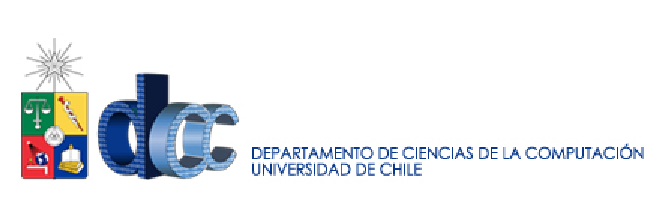
\includegraphics[scale=1]{logo_departamento.eps}
\label{DCC}
\vspace{1cm}
\end{figure}
\begin{center}
\vspace{4cm} {\Huge Tarea 3: Skip Lists y ABB Aleatorizados}

\vspace{1cm} {\Large CC4102 - Diseño y Análisis de Algoritmos}
\vspace{7.5cm}
\end{center}

\begin{tabbing}
\hspace*{7cm}\=\hspace*{3.5cm}\= \kill

\> {\large Profesor:} 	\> 	{\large Gonzalo Navarro} \\ \\
\> {\large Auxiliar:}	\> 	{\large Teresa Bracamonte} \\ \\
\> {\large Alumnos:}	\> 	{\large Cristián Carreño} \\ \\
\> {\large } 			\> 	{\large Sergio Maass} \\ \\
\> {\large Fecha:} 		\> 	{\large 18 de Diciembre de 2013}
\end{tabbing}

\end{titlepage}
%\begin{doublespace}

\tableofcontents
\newpage

\section{Introducción}
Los Skip Lists (SL) son estructuras de datos que permiten almacenar objetos en listas enlazadas ordenadas. A diferencia de las listas enlazadas convencionales, los skip lists aleatorizan el algoritmo de inserción de forma que cada vez que se inserta un nuevo elemento, se pueden generar $d$ duplicados aleatoriamente de forma que estos compongan un atajo para la lista enlazada original y reduzcan el tiempo de búsqueda. La ventaja de los skip list es que aseguran un tiempo promedio de búsqueda de $O(\log{n})$, al igual que los árboles de búsqueda binarios.\\

Los Árboles de Búsqueda Binarios (ABB) aseguran que, en promedio, los tiempo de inserción y búsqueda sean de $O(\log{n})$. Sin embargo, en el peor caso podemos terminar con un árbol de altura $O(n)$. Para reducir ese tipo de situaciones, Martinez y Roura proponen aleatorizar las operaciones de inserción y eliminación en el ABB. Específicamente, en la inserción se considera que cada elemento tiene la probabilidad $\frac{1}{n}$ de ser la raíz del árbol; siendo $n$ el número de elementos actualmente en el árbol.\\

En el presente trabajo se pretende determinar cuál de estas estructuras es mejor en la práctica, para lo cual se implementarán y luego serán sometidas a prueba.

\section{Implementación}
A continuación se detalla la implementación de las estructuras que serán comparadas: Skip List (SL), Árbol Binario de Búsqueda (ABB), y ABB Aleatorizado. Todas se implementaron en Python.

\subsection{Skip List}
\label{sec:sl}

\begin{figure}[ht]
\centering
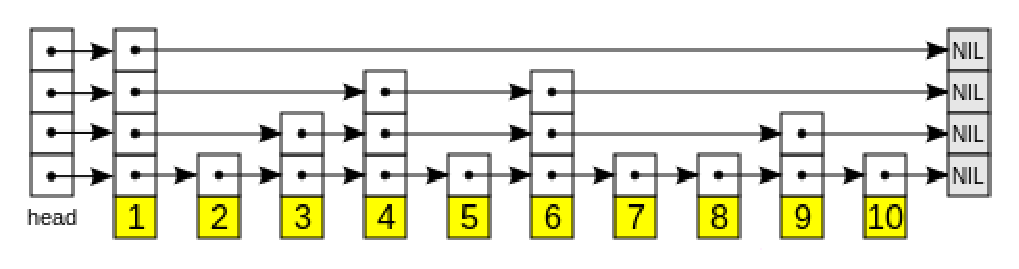
\includegraphics[scale=0.75]{skiplist.eps}
\caption{Estructura de Skip List.}
\label{fig:skip}
\end{figure}

La estructura de una Skip List se aprecia en la figura \ref{fig:skip}. La altura de cada nodo (cantidad de punteros que tiene en listas superiores) se determina del siguiente modo: se elige con probabilidad $\frac{1}{2}$ si el nodo tiene un puntero en el nivel $i$ (comenzando con $i=2$), y en caso afirmativo se procede con la elección para el nivel $i+1$, en caso negativo se termina el proceso. Todo nodo tiene al menos altura $1$ (está presente en la primera lista).\\

Para implementar esta estructura se definieron las clases SkipNode y SkipList.

\subsubsection{Clase SkipNode}
Representa a cada nodo y sus duplicados en listas superiores. Consiste simplemente en una llave $key$ y una lista $next$ de tamaño $n$, donde para cada $i \in [0,n)$, $next_{i}$ es un puntero al siguiente elemento de la i-ésima lista de la Skip List.

\subsubsection{Clase SkipList}
Representa a la lista en sí, la cual está conformada por un SkipNode $head$ y las operaciones de inserción y búsqueda.\\

Ambas operaciones hacen uso del método $closest\_nodes(k)$, el cual entrega una lista de tamaño igual a la altura de la Skip List, y que contiene punteros a los nodos cuyas llaves tienen los valores más cercanos a $k$ por la izquierda (con valor menor a $k$) en cada nivel. El método funciona del siguiente modo:\\

\textbf{closest\_nodes(k)}:
\begin{itemize}
\item	Se crea una lista $u$ de tamaño igual a la altura de la Skip List, inicializada a $None$.
\item	Se asigna $node := head$.
\item	Se itera $i$ desde $|u|$ a $1$:
	\begin{itemize}
	\item	Mientras $node.next[i] \not = None$ y $node.next[i].key < k$
		\begin{itemize}
		\item	$node := node.next[i]$
		\end{itemize}
	\item	$u[i] := node$
	\end{itemize}
\item	Retorna $u$
\end{itemize}

\vspace{0.5cm}
Luego, podemos definir la inserción del siguiente modo:\\

\textbf{insert(k)}:
\begin{itemize}
\item	Se crea un SkipNode $node$ con la llave $k$ que se desea insertar, y una altura determinada con el método explicado en \ref{sec:sl}.
\item	Si la altura de $node$ es mayor a la de $head$, se añaden a $head$ los niveles faltantes (con $None$).
\item	Se obtiene la lista de nodos más cercanos por la izquierda en cada nivel, $u := closest\_nodes(k)$
\item	Para cada nivel $i$ de la altura de $node$:
	\begin{itemize}
	\item	$node.next[i] := u[i].next[i]$
	\item	$u[i].next[i] := node$
	\end{itemize}
\end{itemize}

\vspace{0.5cm}
Finalmente, la búsqueda queda:\\

\textbf{search(k)}:
\begin{itemize}
\item	Se obtiene la lista de nodos más cercanos al valor de $k$ por la izquierda en cada nivel, $u := closest\_nodes(k)$.
\item	Si la longitud de $u$ es mayor que cero:
	\begin{itemize}
	\item	Se asigna $c := u[0].next[0]$ (si el nodo cuya llave es $k$ está en el árbol, ahora será apuntado por $c$).
	\item	Si $c \not = None$ y $c.key = k$, $c$ es el nodo buscado y por ende se retorna.
	\end{itemize}
\item	Si se llegó a este punto la búsqueda fue infructuosa y se retorna $None$.
\end{itemize}

\subsection{ABB}
El ABB se implementó con una clase $Node$ y una clase $ABB$. Cada objeto $Node$ contiene una llave $key$ y los punteros a sus hijos $left$ y $right$. Una instancia de $ABB$ contiene a un objeto $Node$ $root$ y las operaciones $insert$ y $search$. Ambas operaciones consisten en una mera búsqueda binaria, que en el caso de la inserción al encontrar un nodo vacío ($None$) inserta un nuevo nodo en ese espacio. Las operaciones se implementaron de forma iterativa en  vez de recursiva para evitar el desborde de la pila al insertar secuencias ordenadas extensas, ya que Python no provee optimización de llamada por la cola.

\subsection{ABB Aleatorizado}
En cada ABB aleatorizado $T$, debe cumplirse que para todo sub-árbol $T'$ cada nodo tiene probabilidad $\frac{1}{|T'|}$ de ser la raíz, donde $|T'|$ es la cantidad de nodos de $T'$. Esta propiedad se cumple cuando al insertar un nodo en un sub-árbol $T'$, este nodo tiene probabilidad $\frac{1}{|T'|+1}$ de convertirse en la raíz de $T'$. Esto puede lograrse generando un número $n$ pseudoaleatorio distribuido uniformemente entre 0 y $|T'|$, y luego si $n = |T'|$ insertamos al nodo como raíz de $T'$. Para calcular $|T'|$ en cada $T'$ fue necesario agregar el campo $children$ a la clase $Node$, el cual almacena la cantidad de descendientes de este nodo.\\

Para que un nodo se convierta en raíz de un árbol manteniendo la consistencia del mismo lo que se hace es rotarlo desde su posición de inserción hasta que quede en la raíz. A continuación se muestra el algoritmo de inserción, dividido entre la inserción normal y la inserción en la raíz.\\

\textbf{insert(k):}
\begin{itemize}
\item	$self.root := insert\_rec(self.root, k)$
\end{itemize}

\newpage

\textbf{insert\_rec(node, k):}
\begin{itemize}
\item	Si $node = None$, retorna un nuevo nodo de llave $k$.
\item	Si $random(0, node.children + 1) = node.children$
	\begin{itemize}
	\item	Retorna $insert\_at\_root(node, k)$
	\end{itemize}
\item	Si $k < node.key$, $node.left := insert\_rec(node.left, k)$
\item	En caso contrario, $node.right := insert\_rec(node.right, k)$
\item	$node.children := node.children + 1$
\item	Retorna $node$
\end{itemize}

\textbf{insert\_at\_root(node, k):}
\begin{itemize}
\item	Si $node = None$, retorna un nuevo nodo de llave $k$.
\item	Si $k < node.key$:
	\begin{itemize}
	\item	$node.left := insert\_at\_root(node.left, k)$
	\item	$node = rotate\_right(node)$
	\end{itemize}
\item	En caso contrario:
	\begin{itemize}
	\item	$node.right := insert\_at\_root(node.right, k)$
	\item	$node = rotate\_left(node)$
	\end{itemize}
\item	Retorna $node$
\end{itemize}

Las rotaciones de nodo se implementaron según el esquema de la figura \ref{fig:rotaciones}. Estas además actualizan el campo $children$ del nodo rotado.

\begin{figure}[ht]
\centering
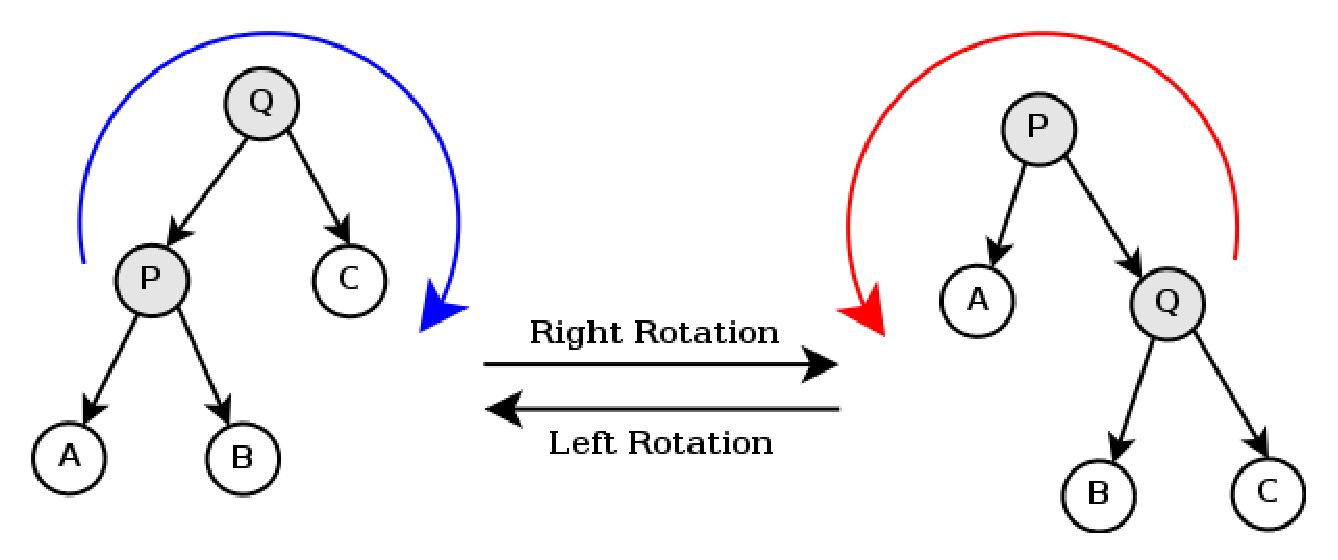
\includegraphics[scale=0.7]{rotations.eps}
\caption{Operaciones de rotación de nodos, hacia la derecha e izquierda.}
\label{fig:rotaciones}
\end{figure}

\section{Experimentos}
Se llevaron a cabo los siguientes experimentos:

\begin{itemize}
\item[1.] Generar una secuencia ordenada de n números; donde $n \in \{10^{4}, 2 \times 10^{4} , 5 \times 10^{4}\}$ y los números corresponden a un subconjunto de enteros entre $[0, 10^{5}]$.
\item[2.] Repetir hasta que, para la secuencia ingresada, se obtenga un comportamiento similar entre los ABB normales y los ABB aleatorizados (se consideró una diferencia de 10\%, es decir, detenerse mientras la cantidad de comparaciones del ABB normal sea mayor en un 10\% a la de un ABB aleatorizado):
	\begin{itemize}
	\item[2.1] Almacenar en cada estructura de datos una secuencia de n números.
		\begin{itemize}
		\item[2.1.1] En los ABB normales se aplican $k$ swaps antes de realizar la secuencia de inserciones; donde $k = 0.005 \times n$. En cada swap se seleccionan aleatoriamente 2 elementos de la secuencia de entrada y se intercambian.
		\end{itemize}
	\item[2.2] Buscar $m$ valores en la estructura de datos; donde $m = 0.5 \times n$ y de los cuales $25\%$ corresponden a búsquedas infructuosas.
	\item[2.3] Utilizar la secuencia obtenida después de aplicar los k swaps en la siguiente iteración.
	\end{itemize}
\end{itemize}

Los resultados se presentan en las secciones siguientes.

\subsection{Tiempos de inserción y búsqueda}

\subsection{Altura promedio de Skip List}

\subsection{Comparación entre ABB y ABB aleatorizado}
Los ABB normales mostraron ser vulnerables a la entrada y alcanzar una cercanía en cuanto a comportamiento a un ABB aleatorizado después de una cantidad cercana a $6/10*n$ en promedio.

\section{Conclusiones}
Los ABB son absolutamente vulnerables al orden en la entrada, y por ende, su convergencia en cuanto a comportamiento se alcanza luego de que el arreglo está completamente desordenado en promedio (la cantidad de swaps necesario para alcanzar este comportamiento es cercano a 7/10*n). Una vez que se alcanza este parecido en comportamiento con los ABB aleatorizados, se puede concluir que se comportan de igual forma, y además, que los ABB aleatorizados son inmunes a la entrada. Las SkipList sin embargo, se comportan mejor que ambas estructuras debido a que su aleatorización tiene una independencia estructural muy grande. Mientras los ABB aleatorizados deben efectuar rotaciones en base a un árbol no perfectamente balanceado las SkipList agregan atajos con cierta probabilidad, lo que, visto a nivel macro, es equivalente a rehacer completamente el árbol y mantener además el invariante de balanceo de hijos. Una SkipList se comporta en promedio de igual forma que un árbol de búsqueda binario perfectamente balanceado lo que implica que su altura es $\altura$ con alta probabilidad.

%\end{doublespace}
\end{document}